\documentclass{standalone}

\usepackage{amsmath,amsfonts,amssymb,amsthm,mathtools} 


\usepackage{fontspec}            % пакет для подгрузки шрифтов
\setmainfont{Arial}   % задаёт основной шрифт документа

% why do we need \newfontfamily:
% http://tex.stackexchange.com/questions/91507/
\newfontfamily{\cyrillicfonttt}{Arial}
\newfontfamily{\cyrillicfont}{Arial}
\newfontfamily{\cyrillicfontsf}{Arial}
% Иногда тех не видит структуры шрифтов. Эти трое бравых парней спасают ситуацию и доопределяют те куски, которые Тех не увидел.

\usepackage{unicode-math}     % пакет для установки математического шрифта
\setmathfont{Asana Math}      % шрифт для математики

\usepackage{polyglossia}      % Пакет, который позволяет подгружать русские буквы
\setdefaultlanguage{russian}  % Основной язык документа
\setotherlanguage{english}    % Второстепенный язык документа




\usepackage{pgf,tikz,pgfplots}
\usetikzlibrary{arrows,calc}
\usepackage{relsize} 

\usepackage{graphicx} 
\usepackage{graphics}
\graphicspath{{Pics/}} 

\usepackage{rotating}
\usepackage{xcolor}
\usepackage{color}


%\definecolor{ydwtaa}{rgb}{160,0,160}
\definecolor{ydwtaa}{HTML}{380049}

\begin{document}

\begin{tikzpicture}[
        scale=2,
        dot/.style={circle,fill=black,minimum size=4pt,inner sep=0pt,
            outer sep=-1pt},
    ]
\node[inner sep=0pt,opacity=0.8] (russell) at (0,0){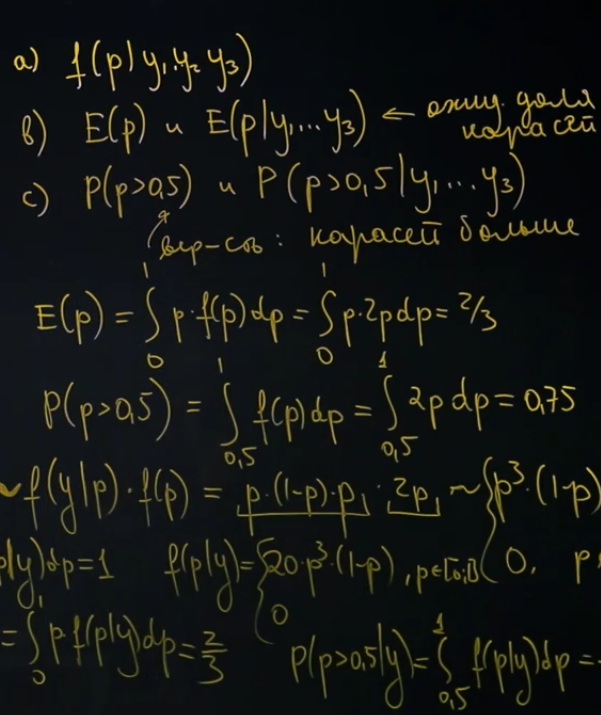
\includegraphics[scale=0.318]{fone_2.png}};     

\draw[fill=white,color=white] (1.8,-1) 
  -- (0,-2.05)
  -- (1.8,-2.05)
  -- cycle;

\draw[fill=white,color=white] (-1.8,-1) 
  -- (0,-2.05)
  -- (-1.8,-2.05)
  -- cycle;

\draw[fill=white,color=white] (0,2.05) 
  -- (-1.8,2.05)
  -- (-1.8,1)
  -- cycle;

\draw[fill=white,color=white] (0,2.05) 
  -- (1.8,2.05)
  -- (1.8,1)
  -- cycle;
  
    
\begin{scope}[rotate=30]       
% Radius of regular polygons
  \newdimen\R
  \R=2cm
  \coordinate (center) at (0,0);
 \draw (0:\R)
     \foreach \x in {60,120,...,360} {  -- (\x:\R) }
              -- cycle (300:\R)
              -- cycle (240:\R)
              -- cycle (180:\R)
              -- cycle (120:\R)
              -- cycle (60:\R)
              -- cycle (0:\R)  [line width=1.9mm,color=ydwtaa];
\end{scope}
                  
% Liza
\node[inner sep=0pt,opacity=1] (russell) at (0,0){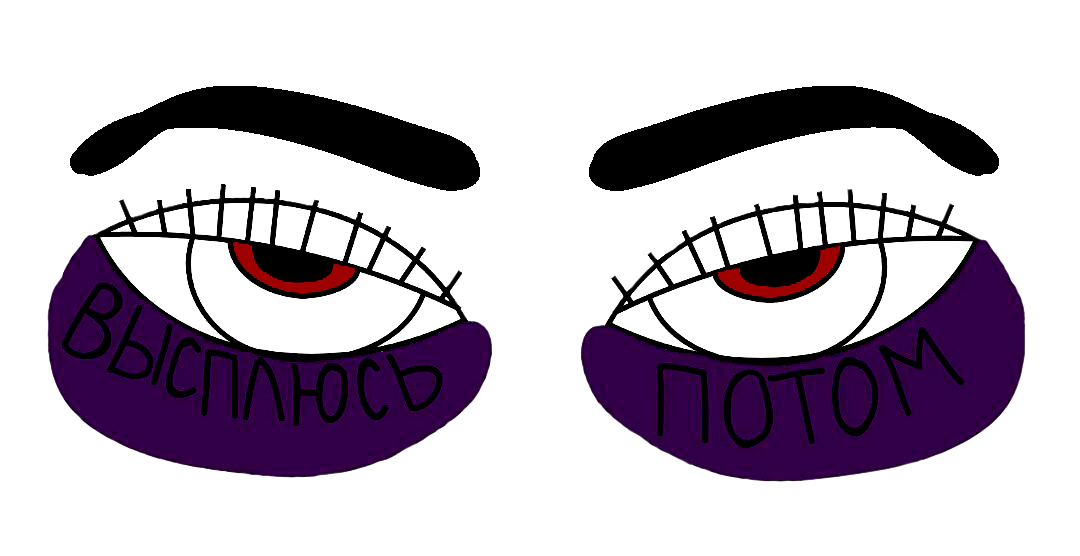
\includegraphics[scale=0.17]{4.png}};   

  
                      
\end{tikzpicture}


\end{document}